\documentclass{article}
\usepackage[margin=2.5cm]{geometry} % Adjust the margin value as desired

\usepackage{amsmath}
\usepackage{amsfonts}

\usepackage{tikz}
\usetikzlibrary {arrows.meta} 
\usepackage{xcolor}
\usepackage{float}

\newcommand{\C}{\mathcal{C}}
\newcommand{\N}{\mathbb{N}}

\title{Models of Computation - Colored Graphs}
\author{Nils Cremer}
\date{\today}

\begin{document}

\maketitle

\section{Motivation}

In this report, I will present a model of computation that I call Colored Graphs.
The motivation behind it is to a more parallel and asynchronous model of computation than let's say the very sequential Turing Machine.
But also to not be restricted by a fixed topology like is the case in cellular automata.
To be able to encode "closeness" of things that belong to each other, e.g. a function and its argument, a graph is natural representation of these kinds of relationships.
Secondly, I wanted the model to be as minimal as I could make it.
It stated out with quite general graph rewriting where large parts of the graph could be added and edges added and removed.
After some simplifications, I ended up with the model that is only comprised of two simple kinds and very local rules.

\section{Colored Graphs}

In this section, I will explain my model of computation which I call Colored Graphs.
It consists of a simple (undirected, no multi-edges, no loops) graph $G = (V, E)$,
together with an edge coloring $c : E \to \C$ that assigns each edge a color from a finite set of Colors $\C$.
You can find an example of a graph below.

\begin{figure}[H]
    \label{fig:graph1}
    \centering
    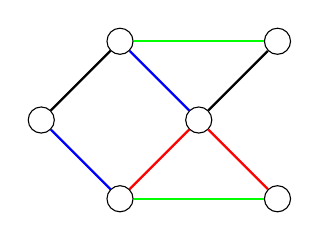
\begin{tikzpicture}
        \node[circle,draw] (A) at (1,-1) {};
        \node[circle,draw] (B) at (2,0) {};
        \node[circle,draw] (C) at (1,1) {};
        \node[circle,draw] (D) at (3,1) {};
        \node[circle,draw] (E) at (3,-1) {};
        \node[circle,draw] (F) at (0,0) {};
        
        \draw[red, thick] (A) -- (B);
        \draw[blue, thick] (B) -- (C);
        \draw[green, thick] (C) -- (D);
        \draw[black, thick] (B) -- (D);
        \draw[green, thick] (E) -- (A);
        \draw[blue, thick] (F) -- (A);
        \draw[black, thick] (F) -- (C);
        \draw[red, thick] (B) -- (E);
    \end{tikzpicture}
    \caption{Example of a Colored Graph}
\end{figure}


The model computes by applying rules to the vertices of a graph which I will first describe informally.
To determine whether a rule can be applied to a vertex of the graph, we look at the colors of incident edges to that vertex.
Concretely, an example rule might apply when a node is incident to 2 red edges and 1 black edge.
When a rule is being applied to a vertex, it changes the graph.
This, however, can not happen in an arbitrary way, but only in two simple ways.
First, the rule can delete the vertex and "rewire" the adjacent vertices, or secondly it can split the vertex in two independent nodes and connected the two vertices to the adjacent vertices of the original vertex.
Next I will describe the rules more formally.

\paragraph*{Delete Rule} A Delete Rule has a condition $b : \C \to \N$.
We say this rule can be applied to a vertex $v$ if the vertex has exactly $b(c)$ incident edges of color $c$ for all $c \in \C$.
If a Delete Rule is applied, the vertex $v$ is deleted and the adjacent vertices rewired.
Since the rule does not distinguish between different neighboring vertices nor different edges of the same color, the rewiring will be of the form "connect the vertices of the blue edges to the vertices of the red edges with a new yellow edge".
Or more formally we have a mapping $d: \C \times \C \rightharpoonup C$, that maps some pairs of colors to a new color.
Note that this in particular also allows a pair of the same color to be mapped to a new color.
This behaves basically in the same way as two different colors, by connecting all vertices connected by this color to each other.
However, no loops will be created, so vertices are not connected to themselves in that case.
In case the Delete Rule connects two vertices that are already connected, the new edge "overwrites" the old edge.

Instead of defining rules completely formally, I will mostly show them visually in the following way where the node the rule is applied to is marked in black.

\begin{center}
    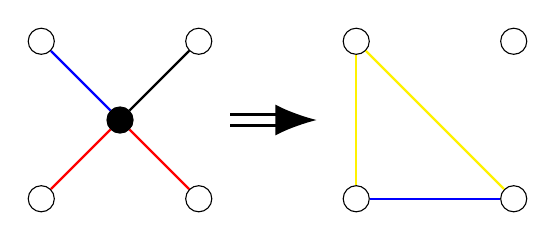
\begin{tikzpicture}
    \begin{scope}[xshift=-2cm]
        \node[circle,draw] (A) at (1,-1) {};
        \node[circle,draw,fill] (B) at (2,0) {};
        \node[circle,draw] (C) at (1,1) {};
        \node[circle,draw] (D) at (3,1) {};
        \node[circle,draw] (E) at (3,-1) {};
        
        \draw[red, thick] (A) -- (B);
        \draw[blue, thick] (B) -- (C);
        \draw[black, thick] (B) -- (D);
        \draw[red, thick] (B) -- (E);
    \end{scope}

    \draw [line width=1pt, double distance=3pt, arrows = {-Latex[length=0pt 3 0]}] (1.4,0) -- (2.5,0);
    
    \begin{scope}[xshift=2cm]
        \node[circle,draw] (A2) at (1,-1) {};
        \node[circle,draw] (C2) at (1,1) {};
        \node[circle,draw] (D2) at (3,1) {};
        \node[circle,draw] (E2) at (3,-1) {};
        
        \draw[blue, thick] (A2) -- (E2);
        \draw[yellow, thick] (A2) -- (C2);
        \draw[yellow, thick] (E2) -- (C2);
    \end{scope}
    \end{tikzpicture}
\end{center}

This represents a Delete Rule that can be applied to a node that had 2 incident red edges, one blue edge and a black edge.
After deletion of the node, it rewires the blue and red vertices with a yellow edge and the red vertices with itself with blue edges.
Notice that I will sometimes call the neighboring vertices "blue vertices" even though the vertices have no color themselves.
This is just shorthand for the vertices that are connected by a blue edge.
The rewiring of the rule above can also be formally describes as the mapping of the pairs of colors $(\text{red}, \text{blue}) \mapsto \text{yellow}$ and $(\text{red}, \text{red}) \mapsto \text{blue}$.

If we apply this rule to the middle vertex of the example graph in Figure \ref{fig:graph1}, we get the following graph.

\begin{figure}[H]
    \label{fig:graph2}
    \centering
    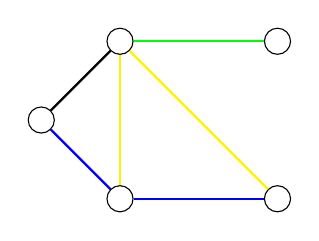
\begin{tikzpicture}
        \node[circle,draw] (A) at (1,-1) {};
        \node[circle,draw] (C) at (1,1) {};
        \node[circle,draw] (D) at (3,1) {};
        \node[circle,draw] (E) at (3,-1) {};
        \node[circle,draw] (F) at (0,0) {};
        
        \draw[green, thick] (C) -- (D);
        \draw[blue, thick] (E) -- (A);
        \draw[blue, thick] (F) -- (A);
        \draw[black, thick] (F) -- (C);
        \draw[yellow, thick] (A) -- (C);
        \draw[yellow, thick] (E) -- (C);
    \end{tikzpicture}
    \caption{Graph after applying the example Delete Rule}
\end{figure}

\paragraph*{Split Rule} A Split Rule has the same kind of condition $b : \C \to \N$ as a Delete Rule.
So again, we count the number of incident edges of each color to see if it matches the condition of the rule.
In contract to a Delete Rule, a Split Rule does not delete the vertex but splits it into two vertices.
The rule then determines which neighboring nodes the two new vertices are connected to.
Again, we don't distinguish vertices that are connected with the same color.
The new connections of the first node can we described by a mapping $s_1 : \C \rightharpoonup \C$ and the new connections of the second node by $s_2 : \C \rightharpoonup \C$.
These mapping describe the colors of the edges with which the two new vertices should be connected to some of the neighboring vertices.

An example Split Rule would be

\begin{center}
    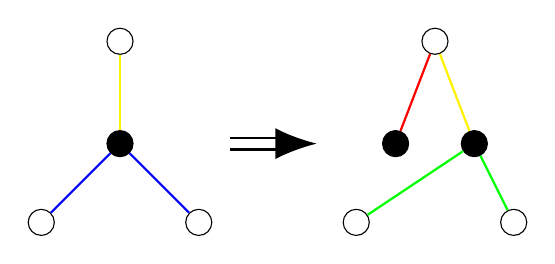
\begin{tikzpicture}
    \begin{scope}[xshift=-2cm]
        \node[circle,draw,fill] (B) at (2,0) {};

        \node[circle,draw] (A) at (1,-1) {};
        \node[circle,draw] (C) at (2,1.3) {};
        \node[circle,draw] (E) at (3,-1) {};
        
        \draw[blue, thick] (B) -- (A);
        \draw[yellow, thick] (B) -- (C);
        \draw[blue, thick] (B) -- (E);
    \end{scope}

    \draw [line width=1pt, double distance=3pt,
             arrows = {-Latex[length=0pt 3 0]}] (1.4,0) -- (2.5,0);
    
    \begin{scope}[xshift=2cm]
        \node[circle,draw,fill] (B2) at (2.5,0) {};
        \node[circle,draw,fill] (D2) at (1.5,0) {};
        
        \node[circle,draw] (A2) at (1,-1) {};
        \node[circle,draw] (C2) at (2,1.3) {};
        \node[circle,draw] (E2) at (3,-1) {};
        
        \draw[yellow, thick] (B2) -- (C2);
        \draw[green, thick] (B2) -- (A2);
        \draw[green, thick] (B2) -- (E2);
        \draw[red, thick] (D2) -- (C2);
    \end{scope}
    
    \end{tikzpicture}
\end{center}

It represents a Split Rule that can be applied to a node that had 2 incident blue edges and one yellow edge.
The two new nodes with their new edges can be described by the mapping $s_1$ that maps yellow to red and $s_2$ which maps blue to green and yellow to yellow.

Applying this rule to the bottom left node in the graph in Figure \ref{fig:graph2}, we get the following graph.

\begin{figure}[H]
    \label{fig:graph3}
    \centering
    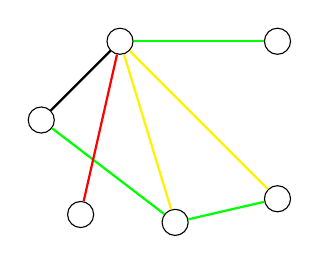
\begin{tikzpicture}
        \node[circle,draw] (A) at (1.7,-1.3) {};
        \node[circle,draw] (C) at (1,1) {};
        \node[circle,draw] (D) at (3,1) {};
        \node[circle,draw] (E) at (3,-1) {};
        \node[circle,draw] (F) at (0,0) {};
        \node[circle,draw] (G) at (0.5,-1.2) {};
        
        \draw[green, thick] (C) -- (D);
        \draw[green, thick] (E) -- (A);
        \draw[green, thick] (F) -- (A);
        \draw[black, thick] (F) -- (C);
        \draw[yellow, thick] (A) -- (C);
        \draw[yellow, thick] (E) -- (C);
        \draw[red, thick] (G) -- (C);
    \end{tikzpicture}
    \caption{Graph after applying the example Split Rule}
\end{figure}

\paragraph*{Computation}
A program in the Colored Graph model is a finite set of Delete and Split Rule.
The input to the model is an initial colored graph.
In each step of the computation an arbitrary rule is applied to a vertex that satisfies the condition of the rule.
This is repeated until no rule can be applied anymore.
Notice that this model is not necessarily confluent meaning that there might be different reductions that lead to different end results.
It is the task of the programmer to design rules and a suitable encoding of the problem input such that the computation always leads to the desired result no matter the order of rule applications.

\section{Example Computations}

To get feel for the model, let's look at some example computations.

\paragraph*{Addition}
Let's try to implement addition in the Colored Graph model.
We represent a number $n$ by a chain of $n+1$ nodes connected to each other with blue edges.
The reason that we use $n+1$ and not $n$ to be able to represent 0 with a single node.
Then to add two number, we will connect the two chains together with a red edge to a long chain.
So the input to our program to add 3 and 5 will be the following graph.

\begin{center}
    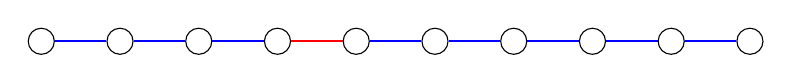
\begin{tikzpicture}
        \node[circle,draw] (A) at (1,0) {};
        \node[circle,draw] (B) at (2,0) {};
        \node[circle,draw] (C) at (3,0) {};
        \node[circle,draw] (D) at (4,0) {};

        \node[circle,draw] (E) at (5,0) {};
        \node[circle,draw] (F) at (6,0) {};
        \node[circle,draw] (G) at (7,0) {};
        \node[circle,draw] (H) at (8,0) {};
        \node[circle,draw] (I) at (9,0) {};
        \node[circle,draw] (J) at (10,0) {};
        
        \draw[blue, thick] (A) -- (B);
        \draw[blue, thick] (B) -- (C);
        \draw[blue, thick] (C) -- (D);
        \draw[red, thick] (D) -- (E);
        \draw[blue, thick] (E) -- (F);
        \draw[blue, thick] (F) -- (G);
        \draw[blue, thick] (G) -- (H);
        \draw[blue, thick] (H) -- (I);
        \draw[blue, thick] (I) -- (J);
    \end{tikzpicture}
\end{center}

To add these two numbers we simply need the following rule.

\begin{center}
    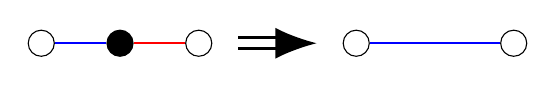
\begin{tikzpicture}
    \begin{scope}[xshift=-2cm]
        \node[circle,draw] (A) at (-1, 0) {};
        \node[circle,draw,fill] (B) at (0,0) {};
        \node[circle,draw] (C) at (1,0) {};
        
        \draw[blue, thick] (A) -- (B);
        \draw[red, thick] (B) -- (C);
    \end{scope}

    \draw [line width=1pt, double distance=3pt, arrows = {-Latex[length=0pt 3 0]}] (-0.5,0) -- (0.5,0);
    
    \begin{scope}[xshift=2cm]
        \node[circle,draw] (A) at (-1, 0) {};
        \node[circle,draw] (C) at (1,0) {};
        
        \draw[blue, thick] (A) -- (C);
    \end{scope}
    \end{tikzpicture}
\end{center}

This rule can be applied to either of the nodes connected to the red edge and in one step will produce the correct restult.

\begin{center}
    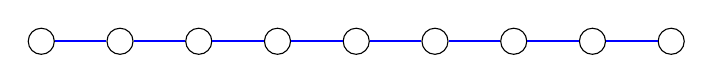
\begin{tikzpicture}
        \node[circle,draw] (A) at (1,0) {};
        \node[circle,draw] (B) at (2,0) {};
        \node[circle,draw] (C) at (3,0) {};
        \node[circle,draw] (D) at (4,0) {};

        \node[circle,draw] (E) at (5,0) {};
        \node[circle,draw] (F) at (6,0) {};
        \node[circle,draw] (G) at (7,0) {};
        \node[circle,draw] (H) at (8,0) {};
        \node[circle,draw] (I) at (9,0) {};
        
        \draw[blue, thick] (A) -- (B);
        \draw[blue, thick] (B) -- (C);
        \draw[blue, thick] (C) -- (D);
        \draw[blue, thick] (D) -- (E);
        \draw[blue, thick] (E) -- (F);
        \draw[blue, thick] (F) -- (G);
        \draw[blue, thick] (G) -- (H);
        \draw[blue, thick] (H) -- (I);
    \end{tikzpicture}
\end{center}

To deal with the special case of $0 + 0$, for which this rule does not work we will add the following Delete Rule that just removes a node connected to exactly one red edge and has an empty rewiring.

\begin{center}
    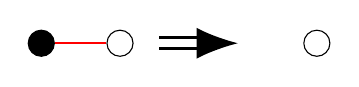
\begin{tikzpicture}
    \begin{scope}[xshift=-2cm]
        \node[circle,draw,fill] (B) at (0,0) {};
        \node[circle,draw] (C) at (1,0) {};
        
        \draw[red, thick] (B) -- (C);
    \end{scope}

    \draw [line width=1pt, double distance=3pt, arrows = {-Latex[length=0pt 3 0]}] (-0.5,0) -- (0.5,0);
    
    \begin{scope}[xshift=2cm]
        \node[circle,draw] (C) at (-0.5,0) {};
    \end{scope}
    \end{tikzpicture}
\end{center}

That was pretty easy so let's turn to some more complex examples.

\paragraph*{Graph vertex connectivity}

As one could image representing graph problems in this model is quite natural.
However, maybe not as natural as one might think.
The main problem is that most graph problems can have graphs with nodes of arbitrary degrees.
Rules in our model can only apply to nodes of a fixed degree though and since we only have finitely many rules, nodes with a very high degree become a problem as no rule could be applied.
The problem we want to solve is to determine whether two nodes $u$ and $v$ in a graph are connected or not.
To encode the graph 



\section{Reduction to Turing Machines}

In this section, I will reduce a Turing Machine $\langle Q, \Sigma, \Gamma, \delta, q_0, q_{halt} \rangle$ to a Colored Graph.
Instead of using actual colors, the set of colors will also contain elements like the states of the Turing Machine.
This makes it clearer which part of the Turing machine is represented by which part of the Colored Graph.
For our Colored Graph we will use the colors $\C = Q \cup \Gamma \cup \{L, R, L', R', end\}$.
I will write the name of the color next to the edges.

First, we need to encode the state of the Turing Machine.
Let $\ldots\sqcup\sqcup x_1 x_2 \ldots x_{i-1} x_{i} x_{i+1} \ldots x_k \sqcup\sqcup\ldots$ be the tape content of the Turing Machine with the head of the Turing machine pointed at $x_i$ and $q$ the current state.
Then we construct the initial Colored Graph as follows.

\begin{center}
    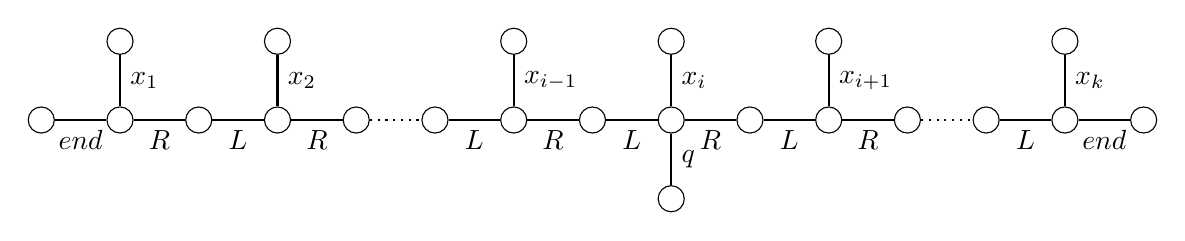
\begin{tikzpicture}
        \node[circle,draw] (A) at (1,0) {};
        \node[circle,draw] (B) at (2,0) {};
        \node[circle,draw] (Bs) at (2,1) {};
        \node[circle,draw] (C) at (3,0) {};
        \node[circle,draw] (D) at (4,0) {};
        \node[circle,draw] (Ds) at (4,1) {};
        \node[circle,draw] (E) at (5,0) {};
        \node[circle,draw] (F) at (6,0) {};
        \node[circle,draw] (G) at (7,0) {};
        \node[circle,draw] (Gs) at (7,1) {};
        \node[circle,draw] (H) at (8,0) {};
        \node[circle,draw] (I) at (9,0) {};
        \node[circle,draw] (Is) at (9,1) {};
        \node[circle,draw] (J) at (10,0) {};
        \node[circle,draw] (K) at (11,0) {};
        \node[circle,draw] (Ks) at (11,1) {};
        \node[circle,draw] (L) at (12,0) {};
        \node[circle,draw] (M) at (13,0) {};
        \node[circle,draw] (N) at (14,0) {};
        \node[circle,draw] (Ns) at (14,1) {};
        \node[circle,draw] (O) at (15,0) {};
        
        \node[circle,draw] (S) at (9,-1) {};
        \draw[thick] (S) -- node[right] {$q$} (I);
        
        \draw[thick] (A) -- node[below] {$end$} (B);
        \draw[thick] (B) -- node[right] {$x_1$} (Bs);
        \draw[thick] (B) -- node[below] {$R$} (C);
        \draw[thick] (C) -- node[below] {$L$} (D);
        \draw[thick] (D) -- node[right] {$x_2$} (Ds);
        \draw[thick] (D) -- node[below] {$R$} (E);
        \draw[thick, dotted] (E) -- node[below] {} (F);
        \draw[thick] (F) -- node[below] {$L$} (G);
        \draw[thick] (G) -- node[below] {$R$} (H);
        \draw[thick] (G) -- node[right] {$x_{i-1}$} (Gs);
        \draw[thick] (H) -- node[below] {$L$} (I);
        \draw[thick] (I) -- node[right] {$x_i$} (Is);
        \draw[thick] (I) -- node[below] {$R$} (J);
        \draw[thick] (J) -- node[below] {$L$} (K);
        \draw[thick] (K) -- node[right] {$x_{i+1}$} (Ks);
        \draw[thick] (K) -- node[below] {$R$} (L);
        \draw[thick, dotted] (L) -- node[below] {} (M);
        \draw[thick] (M) -- node[below] {$L$} (N);
        \draw[thick] (N) -- node[right] {$x_k$} (Ns);
        \draw[thick] (N) -- node[below] {$end$} (O);
    \end{tikzpicture}
\end{center}

The rules to emulate the Turing Machine are as follows.

\begin{itemize}
    \item For each transition $\delta(q, x) = (q', y, R)$ we add the following rule.
    \begin{center}
        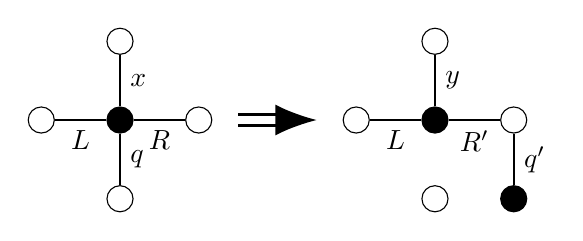
\begin{tikzpicture}
        \begin{scope}[xshift=-2cm]
            \node[circle,draw,fill] (A) at (0, 0) {};
            \node[circle,draw] (B) at (-1,0) {};
            \node[circle,draw] (C) at (0,1) {};
            \node[circle,draw] (D) at (1,0) {};
            \node[circle,draw] (E) at (0,-1) {};
            
            \draw[thick] (A) -- node[below] {$L$} (B);
            \draw[thick] (A) -- node[right] {$x$} (C);
            \draw[thick] (A) -- node[below] {$R$} (D);
            \draw[thick] (A) -- node[right] {$q$} (E);
        \end{scope}
    
        \draw [line width=1pt, double distance=3pt, arrows = {-Latex[length=0pt 3 0]}] (-0.5,0) -- (0.5,0);
        
        \begin{scope}[xshift=2cm]
            \node[circle,draw,fill] (A) at (0, 0) {};
            \node[circle,draw,fill] (A') at (1, -1) {};
            \node[circle,draw] (B) at (-1,0) {};
            \node[circle,draw] (C) at (0,1) {};
            \node[circle,draw] (D) at (1,0) {};
            \node[circle,draw] (E) at (0,-1) {};

            \draw[thick] (A) -- node[below] {$L$} (B);
            \draw[thick] (A) -- node[right] {$y$} (C);
            \draw[thick] (A) -- node[below] {$R'$} (D);
            \draw[thick] (A') -- node[right] {$q'$} (D);
        \end{scope}
        \end{tikzpicture}
    \end{center}
    \item For each transition $\delta(q, x) = (q', y, L)$ we add the following rule.
    \begin{center}
        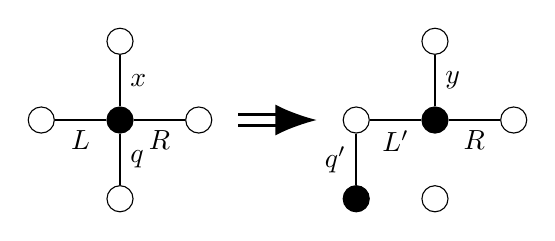
\begin{tikzpicture}
        \begin{scope}[xshift=-2cm]
            \node[circle,draw,fill] (A) at (0, 0) {};
            \node[circle,draw] (B) at (-1,0) {};
            \node[circle,draw] (C) at (0,1) {};
            \node[circle,draw] (D) at (1,0) {};
            \node[circle,draw] (E) at (0,-1) {};
            
            \draw[thick] (A) -- node[below] {$L$} (B);
            \draw[thick] (A) -- node[right] {$x$} (C);
            \draw[thick] (A) -- node[below] {$R$} (D);
            \draw[thick] (A) -- node[right] {$q$} (E);
        \end{scope}
    
        \draw [line width=1pt, double distance=3pt, arrows = {-Latex[length=0pt 3 0]}] (-0.5,0) -- (0.5,0);
        
        \begin{scope}[xshift=2cm]
            \node[circle,draw,fill] (A) at (0, 0) {};
            \node[circle,draw,fill] (A') at (-1, -1) {};
            \node[circle,draw] (B) at (-1,0) {};
            \node[circle,draw] (C) at (0,1) {};
            \node[circle,draw] (D) at (1,0) {};
            \node[circle,draw] (E) at (0,-1) {};

            \draw[thick] (A) -- node[below] {$L'$} (B);
            \draw[thick] (A) -- node[right] {$y$} (C);
            \draw[thick] (A) -- node[below] {$R$} (D);
            \draw[thick] (A') -- node[left] {$q'$} (B);
        \end{scope}
        \end{tikzpicture}
    \end{center}
    \item Next for each $q \in Q$ we add the following two rules.
    \begin{center}
        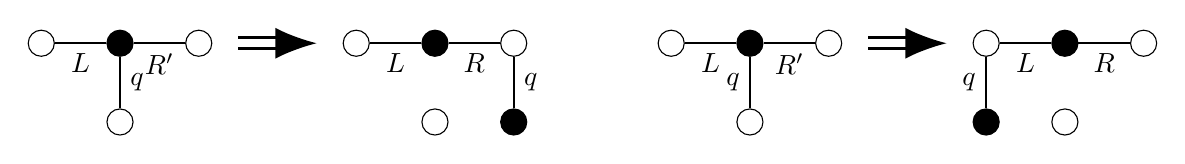
\begin{tikzpicture}
        \begin{scope}[xshift=-4cm]
            \begin{scope}[xshift=-2cm]
                \node[circle,draw,fill] (A) at (0, 0) {};
                \node[circle,draw] (B) at (-1,0) {};
                \node[circle,draw] (D) at (1,0) {};
                \node[circle,draw] (E) at (0,-1) {};
                
                \draw[thick] (A) -- node[below] {$L$} (B);
                \draw[thick] (A) -- node[below] {$R'$} (D);
                \draw[thick] (A) -- node[right] {$q$} (E);
            \end{scope}
        
            \draw [line width=1pt, double distance=3pt, arrows = {-Latex[length=0pt 3 0]}] (-0.5,0) -- (0.5,0);
            
            \begin{scope}[xshift=2cm]
                \node[circle,draw,fill] (A) at (0, 0) {};
                \node[circle,draw,fill] (A') at (1, -1) {};
                \node[circle,draw] (B) at (-1,0) {};
                \node[circle,draw] (D) at (1,0) {};
                \node[circle,draw] (E) at (0,-1) {};
    
                \draw[thick] (A) -- node[below] {$L$} (B);
                \draw[thick] (A) -- node[below] {$R$} (D);
                \draw[thick] (A') -- node[right] {$q$} (D);
            \end{scope}
        \end{scope}

        \begin{scope}[xshift=4cm]
            \begin{scope}[xshift=-2cm]
                \node[circle,draw,fill] (A) at (0, 0) {};
                \node[circle,draw] (B) at (-1,0) {};
                \node[circle,draw] (D) at (1,0) {};
                \node[circle,draw] (E) at (0,-1) {};
                
                \draw[thick] (A) -- node[below] {$L$} (B);
                \draw[thick] (A) -- node[below] {$R'$} (D);
                \draw[thick] (A) -- node[left] {$q$} (E);
            \end{scope}
        
            \draw [line width=1pt, double distance=3pt, arrows = {-Latex[length=0pt 3 0]}] (-0.5,0) -- (0.5,0);
            
            \begin{scope}[xshift=2cm]
                \node[circle,draw,fill] (A) at (0, 0) {};
                \node[circle,draw,fill] (A') at (-1, -1) {};
                \node[circle,draw] (B) at (-1,0) {};
                \node[circle,draw] (D) at (1,0) {};
                \node[circle,draw] (E) at (0,-1) {};
    
                \draw[thick] (A) -- node[below] {$L$} (B);
                \draw[thick] (A) -- node[below] {$R$} (D);
                \draw[thick] (A') -- node[left] {$q$} (B);
            \end{scope}
        \end{scope}
        \end{tikzpicture}
    \end{center}
    \item Since we create isolated vertices with some rules, we add a Delete Rule that just deletes such vertices.
    \begin{center}
        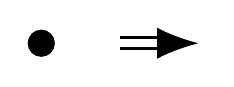
\begin{tikzpicture}
        \begin{scope}[xshift=-1.5cm]
            \node[circle,draw,fill] (A) at (0, 0) {};
        \end{scope}
    
        \draw [line width=1pt, double distance=3pt, arrows = {-Latex[length=0pt 3 0]}] (-0.5,0) -- (0.5,0);
        
        \begin{scope}[xshift=2cm]
        \end{scope}
        \end{tikzpicture}
    \end{center}
    \item Finally, we need some rules to deal with the edges of the tape. For each $x \in \Gamma$ and $q \in Q$ we add the following rules.
    \begin{center}
        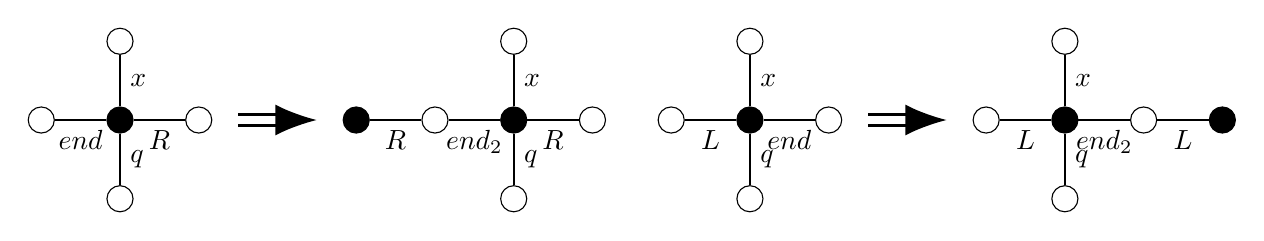
\begin{tikzpicture}
        \begin{scope}[xshift=-4cm]
            \begin{scope}[xshift=-2cm]
                \node[circle,draw,fill] (A) at (0, 0) {};
                \node[circle,draw] (B) at (-1,0) {};
                \node[circle,draw] (C) at (0,1) {};
                \node[circle,draw] (D) at (1,0) {};
                \node[circle,draw] (E) at (0,-1) {};
                
                \draw[thick] (A) -- node[right] {$x$} (C);
                \draw[thick] (A) -- node[right] {$q$} (E);
                \draw[thick] (A) -- node[below] {$end$} (B);
                \draw[thick] (A) -- node[below] {$R$} (D);
            \end{scope}
        
            \draw [line width=1pt, double distance=3pt, arrows = {-Latex[length=0pt 3 0]}] (-0.5,0) -- (0.5,0);
            
            \begin{scope}[xshift=3cm]
                \node[circle,draw,fill] (A) at (0, 0) {};
                \node[circle,draw,fill] (A') at (-2, 0) {};
                \node[circle,draw] (B) at (-1,0) {};
                \node[circle,draw] (C) at (0,1) {};
                \node[circle,draw] (D) at (1,0) {};
                \node[circle,draw] (E) at (0,-1) {};
                
                \draw[thick] (A) -- node[right] {$x$} (C);
                \draw[thick] (A) -- node[right] {$q$} (E);
                \draw[thick] (A) -- node[below] {$end_2$} (B);
                \draw[thick] (A) -- node[below] {$R$} (D);
                \draw[thick] (A') -- node[below] {$R$} (B);
            \end{scope}
        \end{scope}

        \begin{scope}[xshift=4cm]
            \begin{scope}[xshift=-2cm]
                \node[circle,draw,fill] (A) at (0, 0) {};
                \node[circle,draw] (B) at (-1,0) {};
                \node[circle,draw] (C) at (0,1) {};
                \node[circle,draw] (D) at (1,0) {};
                \node[circle,draw] (E) at (0,-1) {};
                
                \draw[thick] (A) -- node[right] {$x$} (C);
                \draw[thick] (A) -- node[right] {$q$} (E);
                \draw[thick] (A) -- node[below] {$L$} (B);
                \draw[thick] (A) -- node[below] {$end$} (D);
            \end{scope}
        
            \draw [line width=1pt, double distance=3pt, arrows = {-Latex[length=0pt 3 0]}] (-0.5,0) -- (0.5,0);
            
            \begin{scope}[xshift=2cm]
                \node[circle,draw,fill] (A) at (0, 0) {};
                \node[circle,draw,fill] (A') at (2, 0) {};
                \node[circle,draw] (B) at (-1,0) {};
                \node[circle,draw] (C) at (0,1) {};
                \node[circle,draw] (D) at (1,0) {};
                \node[circle,draw] (E) at (0,-1) {};
                
                \draw[thick] (A) -- node[right] {$x$} (C);
                \draw[thick] (A) -- node[right] {$q$} (E);
                \draw[thick] (A) -- node[below] {$L$} (B);
                \draw[thick] (A) -- node[below] {$end_2$} (D);
                \draw[thick] (A') -- node[below] {$L$} (D);
            \end{scope}
        \end{scope}
        \end{tikzpicture}

        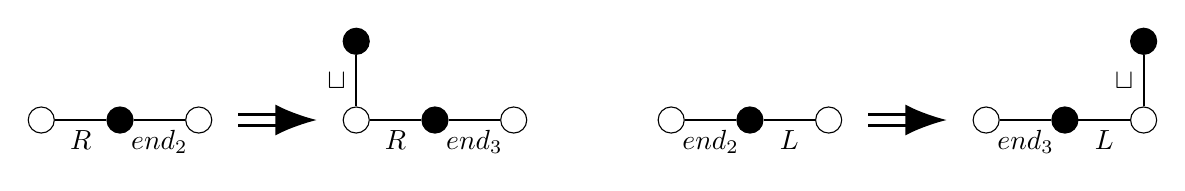
\begin{tikzpicture}
            \begin{scope}[xshift=-4cm]
                \begin{scope}[xshift=-2cm]
                    \node[circle,draw,fill] (A) at (0, 0) {};
                    \node[circle,draw] (B) at (-1,0) {};
                    \node[circle,draw] (D) at (1,0) {};
                    
                    \draw[thick] (A) -- node[below] {$R$} (B);
                    \draw[thick] (A) -- node[below] {$end_2$} (D);
                \end{scope}
            
                \draw [line width=1pt, double distance=3pt, arrows = {-Latex[length=0pt 3 0]}] (-0.5,0) -- (0.5,0);
                
                \begin{scope}[xshift=2cm]
                    \node[circle,draw,fill] (A) at (0, 0) {};
                    \node[circle,draw,fill] (A') at (-1, 1) {};
                    \node[circle,draw] (B) at (-1,0) {};
                    \node[circle,draw] (D) at (1,0) {};
                    
                    \draw[thick] (A) -- node[below] {$R$} (B);
                    \draw[thick] (A) -- node[below] {$end_3$} (D);
                    \draw[thick] (A') -- node[left] {$\sqcup$} (B);
                \end{scope}
            \end{scope}
    
            \begin{scope}[xshift=4cm]
                \begin{scope}[xshift=-2cm]
                    \node[circle,draw,fill] (A) at (0, 0) {};
                    \node[circle,draw] (B) at (-1,0) {};
                    \node[circle,draw] (D) at (1,0) {};
                    
                    \draw[thick] (A) -- node[below] {$end_2$} (B);
                    \draw[thick] (A) -- node[below] {$L$} (D);
                \end{scope}
            
                \draw [line width=1pt, double distance=3pt, arrows = {-Latex[length=0pt 3 0]}] (-0.5,0) -- (0.5,0);
                
                \begin{scope}[xshift=2cm]
                    \node[circle,draw,fill] (A) at (0, 0) {};
                    \node[circle,draw,fill] (A') at (1, 1) {};
                    \node[circle,draw] (B) at (-1,0) {};
                    \node[circle,draw] (D) at (1,0) {};
                    
                    \draw[thick] (A) -- node[below] {$end_3$} (B);
                    \draw[thick] (A) -- node[below] {$L$} (D);
                    \draw[thick] (A') -- node[left] {$\sqcup$} (D);
                \end{scope}
            \end{scope}
            \end{tikzpicture}

            \vspace*{0.8cm}

            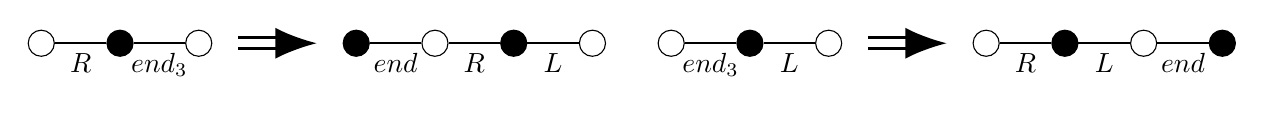
\begin{tikzpicture}
                \begin{scope}[xshift=-4cm]
                    \begin{scope}[xshift=-2cm]
                        \node[circle,draw,fill] (A) at (0, 0) {};
                        \node[circle,draw] (B) at (-1,0) {};
                        \node[circle,draw] (D) at (1,0) {};
                        
                        \draw[thick] (A) -- node[below] {$R$} (B);
                        \draw[thick] (A) -- node[below] {$end_3$} (D);
                    \end{scope}
                
                    \draw [line width=1pt, double distance=3pt, arrows = {-Latex[length=0pt 3 0]}] (-0.5,0) -- (0.5,0);
                    
                    \begin{scope}[xshift=3cm]
                        \node[circle,draw,fill] (A) at (0, 0) {};
                        \node[circle,draw,fill] (A') at (-2, 0) {};
                        \node[circle,draw] (B) at (-1,0) {};
                        \node[circle,draw] (D) at (1,0) {};
                        
                        \draw[thick] (A) -- node[below] {$R$} (B);
                        \draw[thick] (A) -- node[below] {$L$} (D);
                        \draw[thick] (A') -- node[below] {$end$} (B);
                    \end{scope}
                \end{scope}
        
                \begin{scope}[xshift=4cm]
                    \begin{scope}[xshift=-2cm]
                        \node[circle,draw,fill] (A) at (0, 0) {};
                        \node[circle,draw] (B) at (-1,0) {};
                        \node[circle,draw] (D) at (1,0) {};
                        
                        \draw[thick] (A) -- node[below] {$end_3$} (B);
                        \draw[thick] (A) -- node[below] {$L$} (D);
                    \end{scope}
                
                    \draw [line width=1pt, double distance=3pt, arrows = {-Latex[length=0pt 3 0]}] (-0.5,0) -- (0.5,0);
                    
                    \begin{scope}[xshift=2cm]
                        \node[circle,draw,fill] (A) at (0, 0) {};
                        \node[circle,draw,fill] (A') at (2, 0) {};
                        \node[circle,draw] (B) at (-1,0) {};
                        \node[circle,draw] (D) at (1,0) {};
                        
                        \draw[thick] (A) -- node[below] {$R$} (B);
                        \draw[thick] (A) -- node[below] {$L$} (D);
                        \draw[thick] (A') -- node[below] {$end$} (D);
                    \end{scope}
                \end{scope}
                \end{tikzpicture}
    \end{center}
\end{itemize}

\section{Notes on the reduction to Cellular Automata}

My initial plan was to reduce Lambda terms to Colored Graphs.
I made great progress and was able to simulate boolean values, church numerals, addition and multiplication and even pairs.
However, I did not quite finish the reduction as there were always some problem.
I still wanted to make this small section with some notes on my attempt (not only since I spent way too many hours with this but also) because I think there are some interesting ideas and properties I learned.


\end{document}